\subsection{Загрузка файлов}
В данном разделе будет показано, как устанавливать программу и пользоваться ей.
Для описания каждого проделанного шага будут включены описание действий и
скриншоты приложения.

\subsubsection{Установка программы}
Дистрибутив данной программы можно будет получить с прилагаемого CD диска, либо
по ссылке, считав ее с прилагаемого qr-кода(рис.~\ref{ref}).

\begin{figure}[h!]
    \centering
    
\includegraphics[width=0.5\textwidth]{./screenshots/qr.png}
    \caption{ссылка на программу}
    \label{ref}
\end{figure}

Чтобы начать испытания выполнения требований к функциональным характеристикам,
необходимо запустить установщик программы путем выполнения инструкций
(Рис.~\ref{install}), написанных в репозитории данного приложения (ссылка
доступна по qr коду~\ref{ref}).

\begin{figure}[h!]
    \centering
    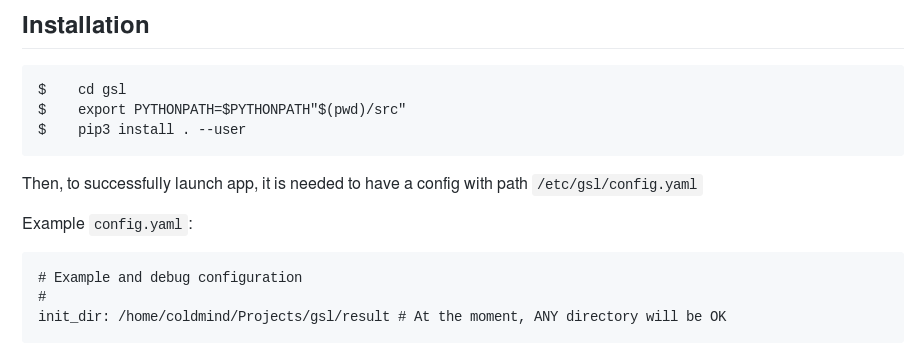
\includegraphics[width=\textwidth]{./screenshots/installation.png}
    \caption{Инструкция по установке программы}\label{install}
\end{figure}

\subsubsection{Использование приложения компоновщик}
Далее приложение необходимо запустить. Запускается компоновщик при помощи команды

\begin{center}
\begin{verbatim}
                                  gsl --init --name myledger --path ~/tmp/gsl
\end{verbatim}
\end{center}

где \emph{myledger} --- название будущего блокчейна, а \emph{~/tmp/gsl} ---
путь до создания директории с блокчейном.

Приложение отобразит приветственное сообщение с вариантами выбора алгоритмов
(пометка 1 на Рис.~\ref{algs_choose}).  Варианты подсвечены в зависимости от
степени поддержки алгоритмов программой (пометка 3 на Рис.~\ref{algs_choose}).
Так же есть возможность выбора значения по умолчанию, не вводя ничего (пометка
2 на Рис.~\ref{algs_choose})

\begin{figure}[h!]
    \centering
    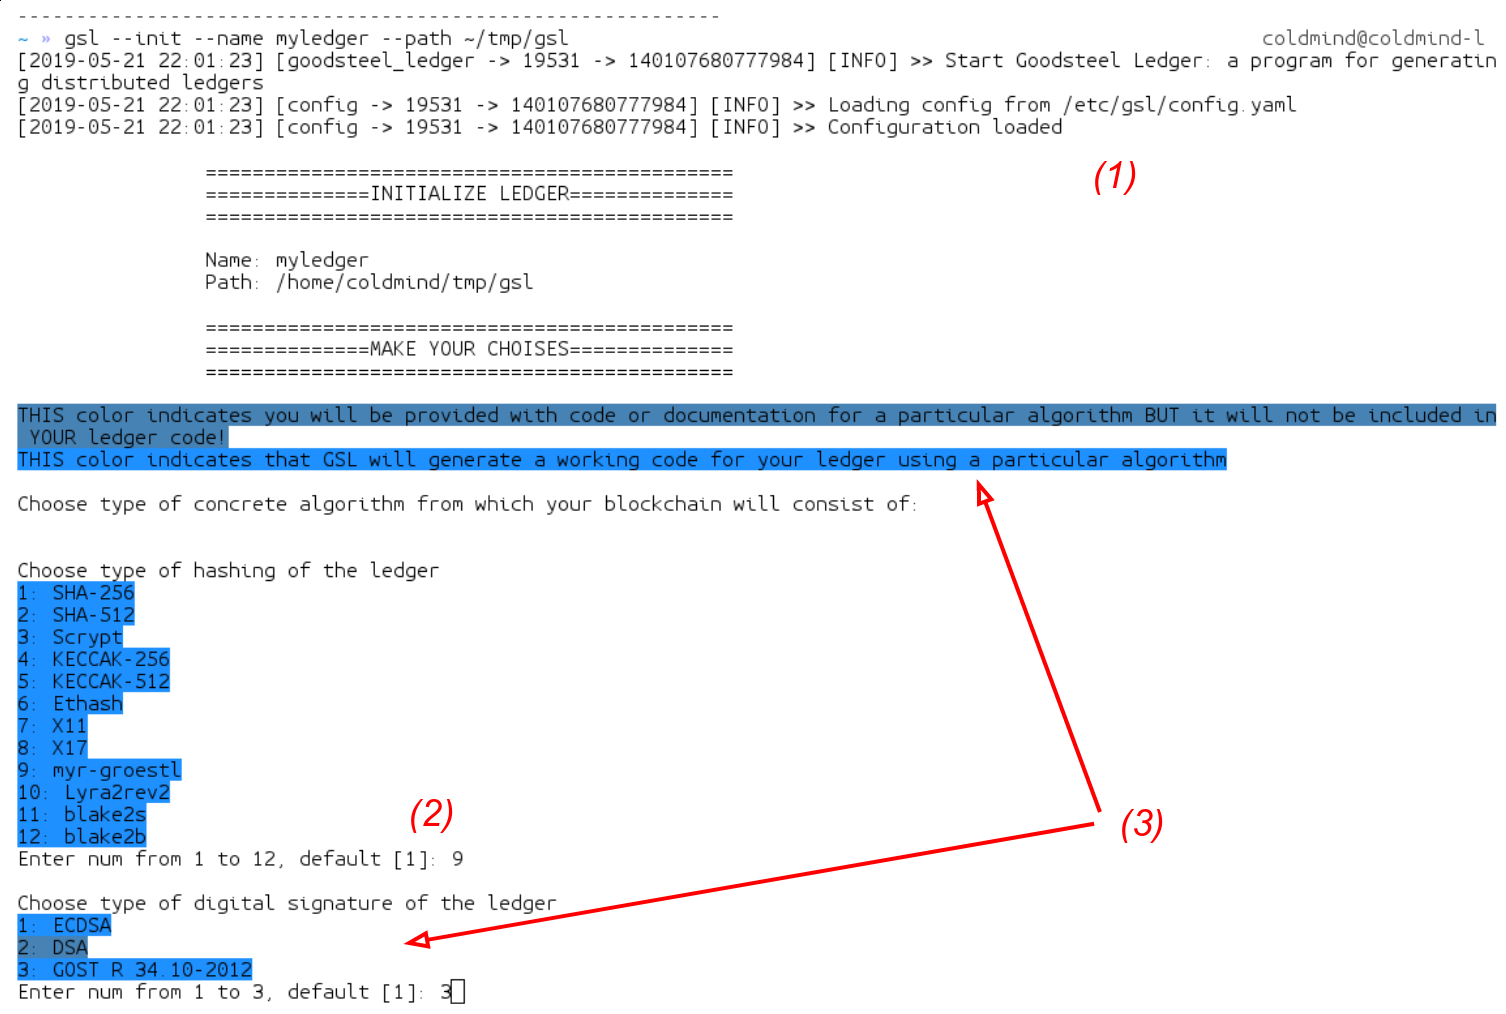
\includegraphics[width=0.85\textwidth]{./screenshots/algs_choose}
    \caption{Начало работы компоновщика}\label{algs_choose}
\end{figure}

После выбора алгоритмов хэширования и цифровой подписи, пользователю
показываются свойства/структура/другие алгоритмы распределённых реестров (Рис.~\ref{additional_opts}), по
которым можно получить справочную информацию (Рис.~\ref{spravka})

\begin{figure}[h!]
    \centering
    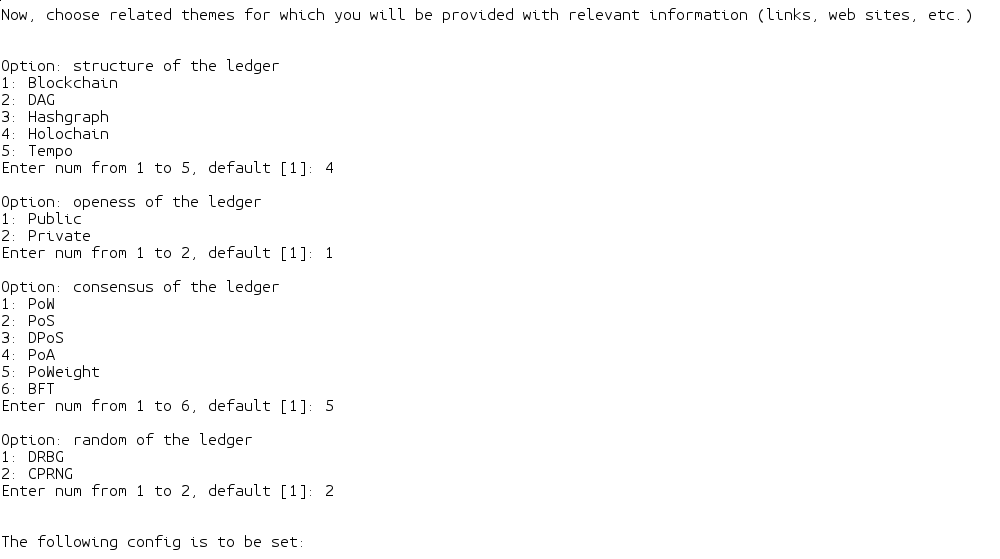
\includegraphics[width=\textwidth]{./screenshots/additional_opts}
    \caption{Вывод опций по которым будет дана справочная информация}\label{additional_opts}
\end{figure}
\begin{figure}[h!]
    \centering
    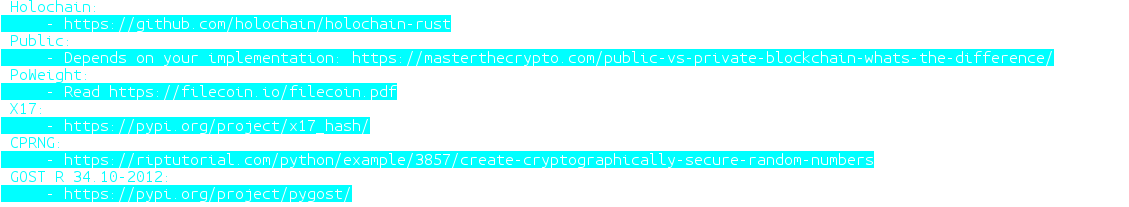
\includegraphics[width=\textwidth]{./screenshots/spravka}
    \caption{Справочная информация в конце выполнения компоновщика}\label{spravka}
\end{figure}

После завершения работы программы по указанной директории располагаются
модули {\small wallet.py} и {\small miner.py} вместе с выбранными алгоритмами
хэщирования и электронной подписи (Рис.~\ref{lldir}).

\begin{figure}[h!]
    \centering
    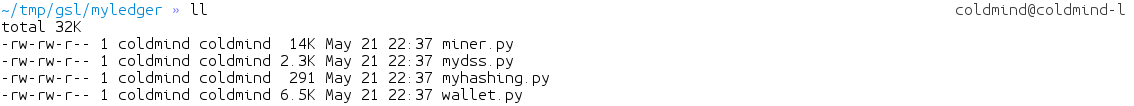
\includegraphics[width=\textwidth]{./screenshots/lldir}
    \caption{директория со сгенерированным кодом}\label{lldir}
\end{figure}

\subsubsection{Использование приложения реализация блокчейна}
Проведём сценарий использования приложения реализация блокчейна. Сгенерируем 2
кошелька, отправим с одного адреса на другой 13 единиц условной валюты

Запустить код кошелька необходимо при помощи команды {\small python3 wallet.py}
и затем выбрать первую опцию. При выборе первой опции должен отображаться
диалог с требованием ввести имя, и дальнейшей генерацией адреса кошелька (пары
публичный-приватный ключи) (Рис.~\ref{gen_kirill_cut}-~-\ref{gen_love})

\begin{figure}[h!]
    \centering
    \minipage{0.49\textwidth}
    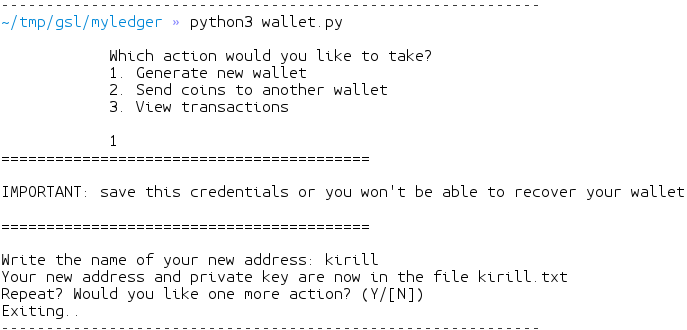
\includegraphics[width=\textwidth]{./screenshots/gen_kirill_cut}
    \caption{Генерация адреса {\small kirill}}\label{gen_kirill_cut}
    \endminipage\hfill
    \minipage{0.49\textwidth}
    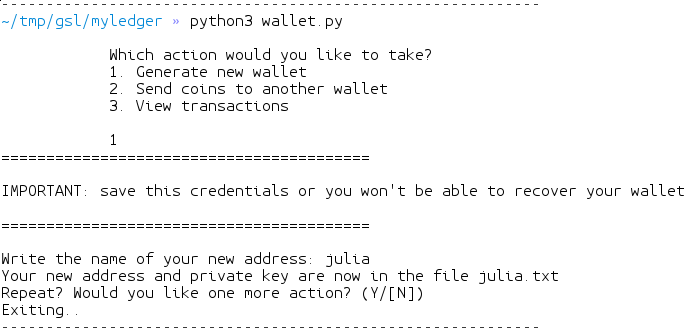
\includegraphics[width=\textwidth]{./screenshots/gen_love}
    \caption{Генерация адреса {\small julia}}\label{gen_love}
    \endminipage{}
\end{figure}

Таким образом, были сгенерированы 2 адреса кошельков (Рис.~\ref{cat_hash})
\begin{figure}[h!]
    \centering
    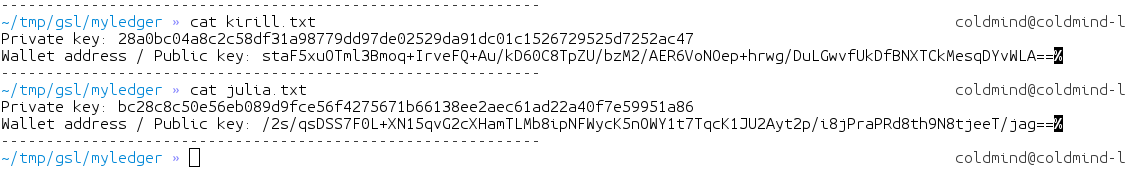
\includegraphics[width=\textwidth]{./screenshots/cat_hash}
    \caption{Адреса кошельков}\label{cat_hash}
\end{figure}
Теперь можно приступать к отправке условных средств с одного адреса на адрес
другой. В другом окне запустить майнер командой {\small python3 miner.py}, и
оставить его исполнение.

При запуске майнера, должен вестись лог о проведённых транзакциях и их
валидациях (Рис.~\ref{log1}~-~Рис.~\ref{log2}).

\begin{figure}[h!]
    \centering
    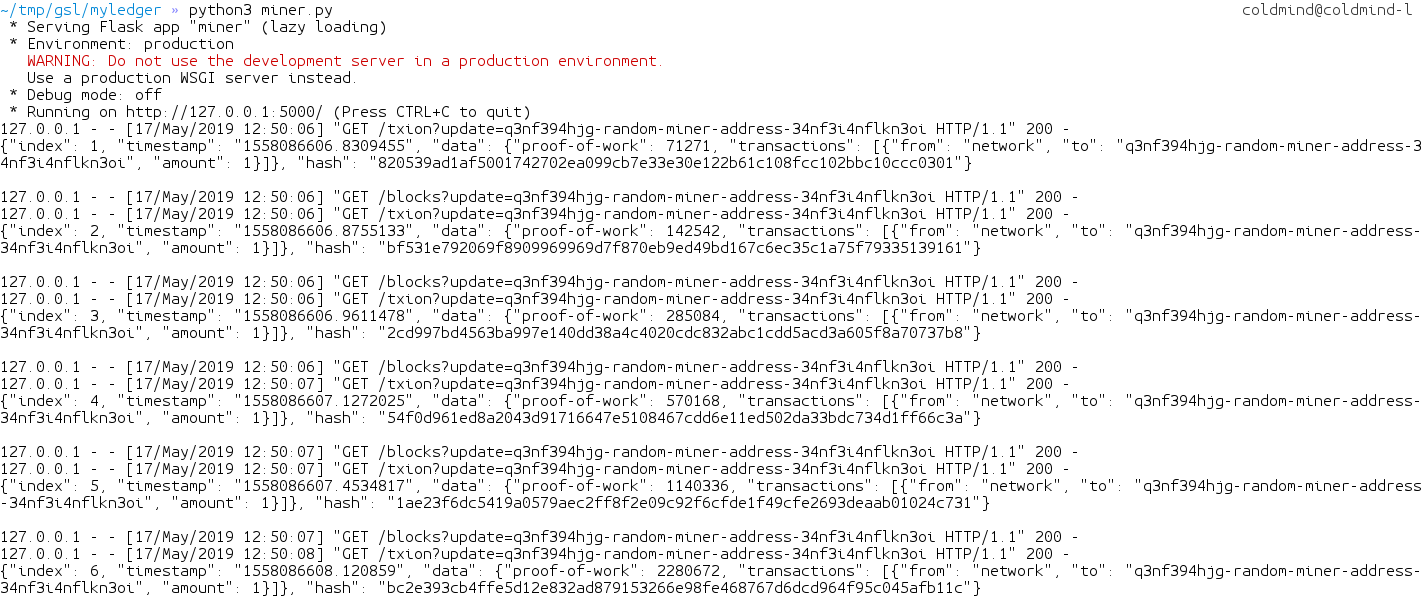
\includegraphics[width=\textwidth]{./screenshots/miner_run}
    \caption{Лог работы майрена}\label{log1}
\end{figure}

В кошельке для отправке условных средств с одного счёта на другой, необходимо
выбрать вторую опцию и ввести публичный и приватный адреса отправителя, а так
же публичный ключ получателя (Рис.~\ref{sending}). Подтвердить намерение
отправить и осуществить тем самым отправку.

\begin{figure}[h!]
    \centering
    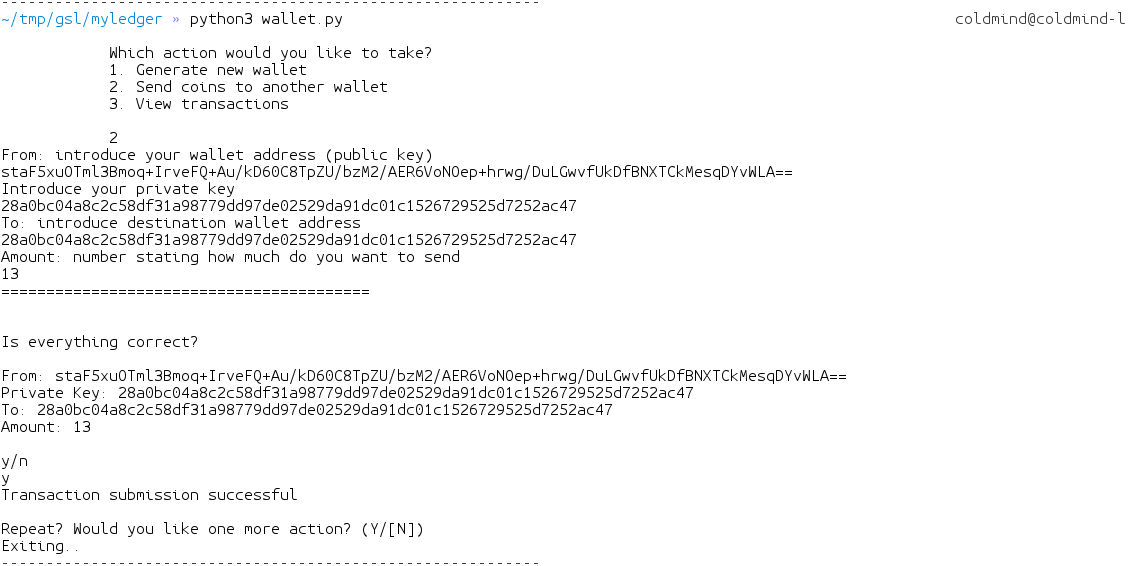
\includegraphics[width=\textwidth]{./screenshots/sending_sha}
    \caption{Процесс отправки средств}\label{sending}
\end{figure}
\begin{figure}[h!]
    \centering
    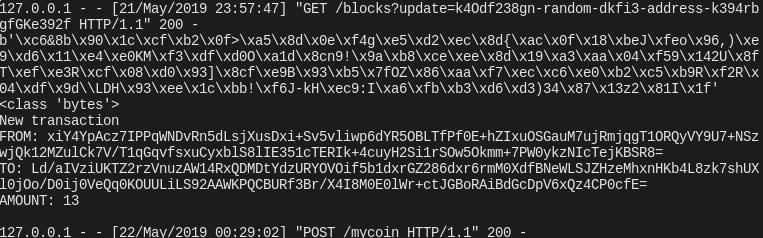
\includegraphics[width=\textwidth]{./screenshots/log_send}
    \caption{Лог регистрации новой транзакции}\label{log2}
\end{figure}

Теперь, можно проверить весь блокчейн на предмет совершённой транзакции. При
выборе третей опции в кошельке, должен отобразиться полная цепочка
транзакций (блокчейн) (Рис.~\ref{full_chain}).
\begin{figure}[h!]
    \centering
    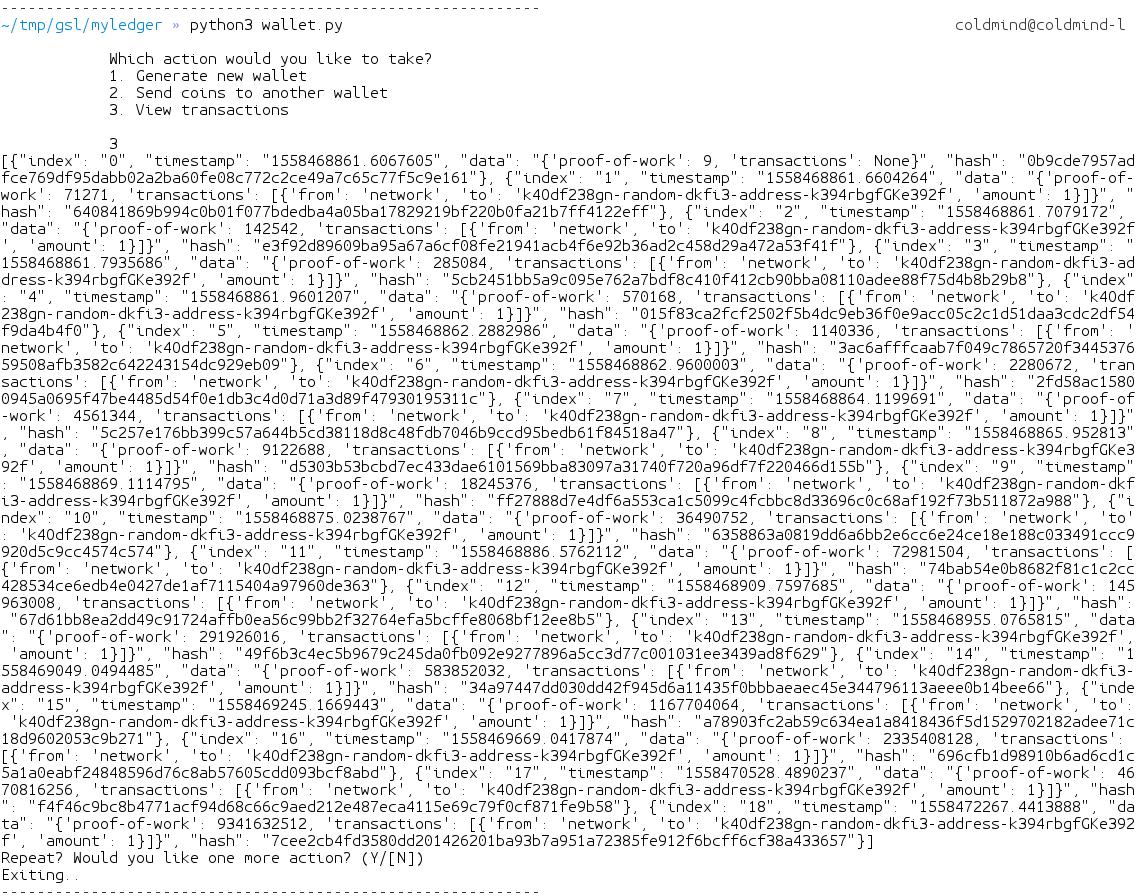
\includegraphics[width=\textwidth]{./screenshots/full_chain}
    \caption{Отображение полной цепочки транзакций}\label{full_chain}
\end{figure}

На этом работу программы можно считать завершённой.
\newpage
